\documentclass[9pt]{IEEEtran}

\usepackage[english]{babel}
\usepackage{graphicx}
\usepackage{epstopdf}
\usepackage{fancyhdr}
\usepackage{amsmath}
\usepackage{amsthm}
\usepackage{amssymb}
\usepackage{url}
\usepackage{array}
\usepackage{textcomp}
\usepackage{listings}
\usepackage{hyperref}
\usepackage{xcolor}
\usepackage{colortbl}
\usepackage{float}
\usepackage{gensymb}
\usepackage{longtable}
\usepackage{supertabular}
\usepackage{multicol}

\usepackage[utf8x]{inputenc}

\usepackage[T1]{fontenc}
\usepackage{lmodern}
\input{glyphtounicode}
\pdfgentounicode=1

\graphicspath{{./figures/}}
\DeclareGraphicsExtensions{.pdf,.png,.jpg,.eps}

% correct bad hyphenation here
\hyphenation{op-tical net-works semi-conduc-tor trig-gs}

% ============================================================================================

\title{\vspace{0ex}
Classification trees, random forests}

\author{Marko Medved\vspace{-4.0ex}}

% ============================================================================================

\begin{document}

\maketitle

\section{Part 1: Implementing classification trees and random forests}
\subsection{Implementation details}

When building a decision tree, the main task is to decide on the splits of the data space. To implement
 this, we start by considering each feature individually. For each feature, the goal is to find the best 
 threshold for the split. To do this, the feature column and the corresponding labels are sorted by the 
 feature values. Then, four counters are defined: two for the count of 0s and 1s in the first split, and
  another two for the count of 0s and 1s in the second split. Since the feature is sorted, the counters are
   simply updated according to the label at the current feature value. For example, if 
y=1, the counter of ones in the first split increases by one, and the counter of ones in the second split is decreased by 1. For each possible threshold, which is set to the average of the current and next feature values, the probabilities are calculated using the counters. For example, the probability of 0 in the first split of the space is calculated as 
$\frac{\text{counter of zeros in the first space}}{\text{counter of ones in the first space}
 + \text{counter of zeros in the first space}}$. Based on these probabilities, a cost function is
  defined using a weighted sum (weighted by the number of data points in each split) of Gini impurities.
   If the calculated cost is lower than the current lowest cost, the lowest cost is updated along with the 
   feature and threshold, that are used for splitting. If the cost is the same as the current lowest cost, the values are not updated, 
   which introduces a slight bias toward the beginning features. 
\\

In the random forest implementation, a specified number of trees ($n$) 
are constructed. Each tree is built using a bootstrapped sample of the training data.
 During each split, only a randomly selected subset  $\sqrt{n}$ features is considered. For making
  predictions, the random forest takes the majority vote from all the trees.

\subsection{Classification results of the tree and random forest models} 
The classification results are presented with the misclassification rate and its uncertainty, 
calculated by bootstrapping the prediction errors (computed as $|y - y_{prediction}|$).
 The misclassification rate was calculated for each of the 1000 bootstrap samples, and the uncertainty
  was estimated as the standard deviation of these misclassification rates. 
 The results can be observed in Table ~\ref{tab:results}.  


 \begin{table}[h]
    \begin{tabular}{l|l}
    Model                           & Missclasification           \\
    \hline
    Classification Tree (Train set) & 0.0 $\pm$ 0.0                 \\
    Classification Tree (Test set)  & 0.300 $\pm$ 0.059  \\
    Random Forest (Train set)       & 0.0 $\pm$ 0.0                 \\
    Random Forest (Test set)        & 0.200 $\pm$ 0.052
    \end{tabular}
    \vspace{2px}
    \caption{Classification Tree and Random Forest missclassification results}
    \label{tab:results}
\end{table}

Furhermore the missclassification rate changes with the number of trees in random forest.
Figure~\ref{fig:missclass_num_trees} shows that relation, including the missclassification uncertainty. 

\begin{figure}[h]
    \centering
    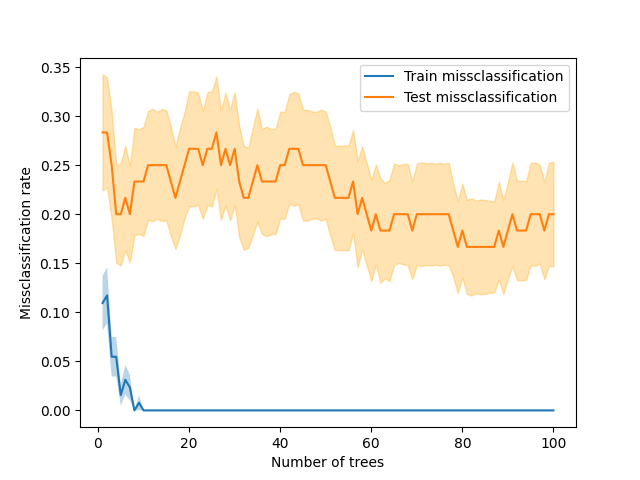
\includegraphics[width=0.95\columnwidth]{figures/missclass_num_trees.png}
    \caption{Misclassification versus the number of trees.}
    \label{fig:missclass_num_trees}
\end{figure}

\section{Part 2: Permutation based variable importance}
Permutation-based variable importance in a random forest is calculated by measuring the drop in 
classification accuracy when permuting each feature's values. For each tree, only the features used by 
that tree are considered; features not used are immediately assigned an importance of zero since permuting 
them will not affect accuracy. The drop in accuracy is evaluated using out-of-the-bag (OOB) data — 
the samples not used to build the current tree due to bootstrap sampling. The importance scores from each 
tree are then averaged across all trees in the forest to obtain the final importance for each feature. Note that 
the Random Forest was built with 100 trees. 
\\

Figure~\ref{fig:importances} shows the permutation-based variable importance along with a comparison to the 
features that appear at the roots of trees and the respective number of times they appear in the root.
Note that when identifying the roots of the trees, all features were included, and the trees were built as full trees.

\begin{figure}[h]
    \centering
    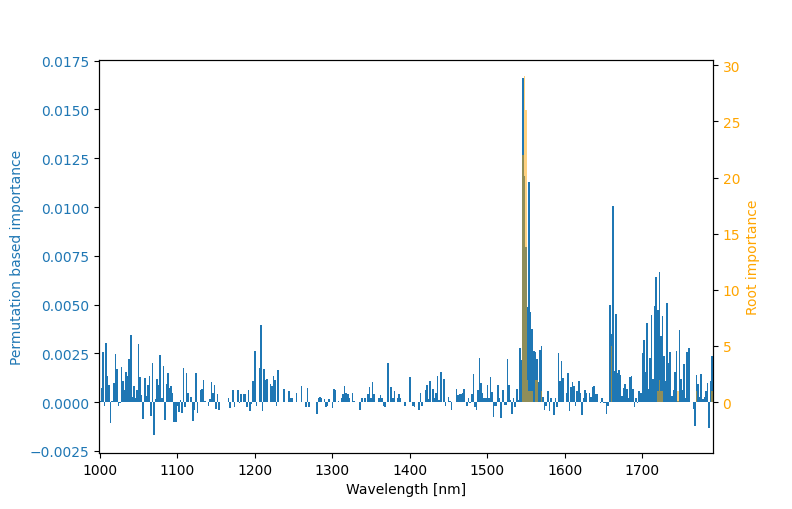
\includegraphics[width=0.95\columnwidth]{figures/importances.png}
    \caption{Feature importances using permutation based importance as well as number of times the feature
    appears in the root of the tree.}
    \label{fig:importances}
\end{figure}

\section{Part 3: Calculating importance of combinations of 3 variables}
\subsection{Permutation importance}
This importance was calculated using the same method as in the previous part, but with one key difference: 
here, all combinations of three features were considered, and for each combination, all three features were 
permuted simultaneously. 
\\
In Table~\ref{tab:results-importances}, we compare the two different methods of calculating 
feature importance. For the comparison, a classification tree was built using the top three features
 from each importance calculation variant. The uncertainty was calculated in the same way as previously. Note
  that the missclassification is lower in the importance3 case, which is not surprising since the best features 
  according to the normal importance method are really close together in the Fourier spectrum, hence they are 
  highly correlated with each other. 

\begin{table}[h]
    \centering
    \begin{tabular}{l|l}
        Importance variant                           & Misclassification           \\
        \hline
        Importance & 0.383$\pm$ 0.065                \\
        Importance3   & 0.350 $\pm$  0.062
    \end{tabular}
    \vspace{2px}
    \caption{Comparison of tree misclassification using the top three features of both importance calculation variants}
    \label{tab:results-importances}
\end{table}

\subsection{Tree structure importance}
Another algorithm was designed to calculate the importance of feature combinations in Random Forests.
 In this approach, each time a feature appears in the structure of a tree, it is assigned a fraction of 
 importance. Specifically, the importance added is $1/2^D$ of importance, where $D$ is the depth of the node.
 The exponential decline in importance with depth is justified by the fact that, on average, each decision 
 at a given level affects,  only half the amount of data points as one level above.
  This calculation is 
  done for every tree in the forest. For each tree, only the top three features with the highest importance
   are considered, and their individual importances are summed to determine their joint importance. The importances of 
   those triples are then summed up across the entire forest.
   \\

   This method is based on the premise that decisions made higher in the tree structure are more 
   significant for the model. Since the top three features in each tree contribute the most to the model, 
   they represent the best combination of features for that tree. By summing their importances, we obtain the highest 
   importance for the best combination of three features. 
    \\


%    \begin{table}[h]
%        \centering
%        \begin{tabular}{l|l|l}
%             Rank & Permutation Triple [nm]&   Tree structure triple [nm]   \\
%             \hline
%             1 &  1786, 1720, 1548    &    1658,1546, 1116        \\
%             2   &  1760, 1702, 1218 & 1718, 1654, 1246 \\
%             4   &  1726, 1268, 1230 & 1608, 1562, 1552 \\
%             4   &  1720, 1296, 1130 & 1748, 1552, 1316 \\
%             5   &  1784, 1540, 1506 & 1638, 1546, 1426 \\

%         \end{tabular}
%         \vspace{2px}
%         \caption{Comparison of top 3 features of both importance3 variants}
%         \label{tab:importance3-comparison}
%     \end{table}

\end{document}
